\documentclass{article}

% if you need to pass options to natbib, use, e.g..
\PassOptionsToPackage{numbers, compress}{natbib}
% before loading neurips_2026

% The authors should use one of these tracks.
% Before accepting by the NeurIPS conference, select one of the options below.
% === SIMBIOCHEM II (NeurIPS 2026 workshop) ===
% SIMBIOCHEM II is a double-blind, non-archival workshop. Use this for submission.
\usepackage[dblblindworkshop]{neurips_2026}
% line numbers are a submission convention; enabled by default for review (kept per user preference)
% For the camera-ready (accepted) version, switch to.
%   \usepackage[dblblindworkshop, final]{neurips_2026}
% This sets the footer, which on the camera-ready reads.
%   "Accepted as a Workshop Paper at the 2nd SIMBIOCHEM, NeurIPS 2026."
\workshoptitle{2nd SIMBIOCHEM Workshop at NeurIPS 2026}
% ---
% the "default" option is equal to the "main" option, which is used for the Main Track with double-blind reviewing.
% 1. "main" option is used for the Main Track
%  \usepackage[main]{neurips_2026}
% 2. "position" option is used for the Position Paper Track
%  \usepackage[position]{neurips_2026}
% 3. "eandd" option is used for the Evaluations & Datasets Track
 % \usepackage[eandd]{neurips_2026}
% 4. "creativeai" option is used for the Creative AI Track
%  \usepackage[creativeai]{neurips_2026}
% 5. "sglblindworkshop" option is used for the Workshop with single-blind reviewing
 % \usepackage[sglblindworkshop]{neurips_2026}
% 6. "dblblindworkshop" option is used for the Workshop with double-blind reviewing
%  \usepackage[dblblindworkshop]{neurips_2026}
% 7. "education" option is used for the Education Track
%  \usepackage[education]{neurips_2026}

% After being accepted, the authors should add "final" behind the track to compile a camera-ready version.
% 1. Main Track
 % \usepackage[main, final]{neurips_2026}
% 2. Position Paper Track
%  \usepackage[position, final]{neurips_2026}
% 3. Evaluations & Datasets Track
 % \usepackage[eandd, final]{neurips_2026}
% 4. Creative AI Track
%  \usepackage[creativeai, final]{neurips_2026}
% 5. Workshop with single-blind reviewing
%  \usepackage[sglblindworkshop, final]{neurips_2026}
% 6. Workshop with double-blind reviewing
%  \usepackage[dblblindworkshop, final]{neurips_2026}
% Note. For the workshop paper template, both \title{} and \workshoptitle{} are required, with the former indicating the paper title shown in the title and the latter indicating the workshop title displayed in the footnote.
% For workshops (5., 6.), the authors should add the name of the workshop, "\workshoptitle" command is used to set the workshop title.
% \workshoptitle{WORKSHOP TITLE}
% 7. Education Track
% \usepackage[education, final]{neurips_2026}

% "preprint" option is used for arXiv or other preprint submissions
 % \usepackage[preprint]{neurips_2026}

% to avoid loading the natbib package, add option nonatbib.
%    \usepackage[nonatbib]{neurips_2026}

\usepackage[utf8]{inputenc} % allow utf-8 input
\usepackage[T1]{fontenc}    % use 8-bit T1 fonts
\usepackage{hyperref}       % hyperlinks
\hypersetup{pdfauthor={}}   % keep PDF metadata anonymous under double-blind review
\usepackage{url}            % simple URL typesetting
\usepackage{booktabs}       % professional-quality tables
\usepackage{amsfonts}       % blackboard math symbols
\usepackage{amsmath}        % \text{} inside math (needed by our math notation)
\usepackage{nicefrac}       % compact symbols for 1/2, etc.
\usepackage{microtype}      % microtypography
\usepackage{xcolor}         % colors
\usepackage{graphicx}       % figures
\usepackage{times}
% Note. For the workshop paper template, both \title{} and \workshoptitle{} are required, with the former indicating the paper title shown in the title and the latter indicating the workshop title displayed in the footnote.
\title{Shrinkage Needs a Gauge: Identifiability and Test-Time Correction of Additive Molecular Energy Predictions}

% The \author macro works with any number of authors. There are two commands
% used to separate the names and addresses of multiple authors. \And and \AND.
%
% Using \And between authors leaves it to LaTeX to determine where to break the
% lines. Using \AND forces a line break at that point. So, if LaTeX puts 3 of 4
% authors names on the first line, and the last on the second line, try using
% \AND instead of \And before the third author name.

% Author block. real author info (source-only; not rendered under
% dblblindworkshop without final/preprint). Anonymity for the review copy is
% handled by the style file; PDF metadata is suppressed via \hypersetup above.



\begin{document}

\maketitle

\begin{abstract}
  Hydration free energy, the free energy of moving a molecule from vacuum
  into water, is central to drug design, and graph networks now predict it
  within a few tenths of a kcal/mol on FreeSolv. Average accuracy is not
  enough for deployment, because a model must know when it is wrong on a
  single molecule. The standard tool is ensemble disagreement, yet on FreeSolv
  it fails concretely, with 18 of 129 fold-0 test molecules (14\%) confidently
  wrong despite agreement among members. Rather than detecting these cases, we
  correct them by shrinking per-atom energy contributions toward a
  cross-molecular pool mean at test time. The natural atom-level weighting by
  per-atom variance has a hidden flaw, because the additive decomposition of a
  molecular energy is not unique. A zero-sum, seed-independent reallocation
  across atoms leaves the molecular prediction and per-atom variances unchanged
  but still changes the variance-weighted correction. We introduce
  Gauge-Invariant Molecular Shrinkage (GIMS), which aggregates atomic
  reliability into one molecule-level strength and shrinks the molecular total,
  making it exactly invariant to the reallocation. GIMS beats a matched-strength
  uniform baseline significantly on four of five test populations, both on the
  main test and on a held-out H2 split, and beats variance-weighted shrinkage
  in point estimate on all five populations, though not yet significantly.
  Under the same null reallocation VW shifts by 3.26~kcal/mol on average while
  GIMS shifts by $\sim 2.5\times10^{-14}$. Retrained on the frozen split, the
  model transfers to 620 external molecules at MAE 1.475 ($R^2$ 0.854), a
  2.5$\times$ degradation from the same-run anchor consistent with domain shift.
  Flat GIMS does not transfer there, while a tiny affine recalibration restores
  a small consistent gain.
\end{abstract}
% VERIFIED. 18/129=14\% quadrant split = deep_ensemble/rmse_analysis/analyze_std_vs_rmse.py; ext. MAE 1.475 R2 0.854 = verification/expdb_external/results/expdb_conformers.hdf5 run; GIMS vs uniform significant on 4/5 (see Results); gauge VW 3.26 vs GIMS 2.49e-14 = node_refinement/gauge_invariant_shrinkage/gims_report.json:gauge_stress and GAUGE_INVARIANT_SHRINKAGE_RESULTS.md.

\section{Introduction}

The hydration free energy of a small molecule, the free energy of
transferring it from vacuum into water, is central to drug discovery~\cite{mobley2014freesolv}.
It can be estimated with physics (force fields, GBn2, COSMO-RS) or learned
from FreeSolv (642 values). Graph networks now reach a few tenths of a kcal/mol~\cite{zhang2022}.
% VERIFIED. \cite{zhang2022} = Zhang, Xia, Zhang, JCIM 62(8):1840-1848, 2022
% (A3D-PNAConv-FT; FreeSolv MAE 0.417 / RMSE 0.719, random splits). bibitem added.

Average accuracy is not enough for deployment, because decisions are made per
molecule and a model that is right on average can still be wrong on the
compound at hand. Uncertainty quantification is therefore a separate problem
from accuracy.

The standard tool is ensemble disagreement, where different seeds give
different members and their spread is used as uncertainty. We test this on
FreeSolv with a DimeNet++ model pretrained on Aquamarine (59{,}783
conformers of 1{,}653 molecules)~\cite{medranosandonas2024aquamarine} and
fine-tuned on FreeSolv, and find that 18 of 129 test molecules (14\%) are
confidently wrong under the 5-seed spread, with members in agreement yet
predictions inaccurate. Structural isolation explains six, while feature density
explains none of the remaining twelve, and a cutoff-radius explanation is also
ruled out, as bias magnitude is uncorrelated with size and confidently-wrong
molecules are not large.
% VERIFIED. 18/129 quadrant split = deep_ensemble/rmse_analysis/analyze_std_vs_rmse.py; ext. 620 MAE 1.475 as in Abstract; cutoff null = node_refinement/cutoff_bias_check/cutoff_bias_check.py and docs/progress/CUTOFF_BIAS_CHECK_RESULTS.md.

An alternative to detection is correction. DimeNet++ predicts a molecular
energy as a sum of per-atom contributions that can be shrunk toward a
cross-molecular pool mean at test time, and weighting that shrinkage by
per-atom variance seems natural. It has a hidden flaw, because the additive
decomposition is not unique. A zero-sum, seed-independent shift across atoms
leaves the molecular prediction and per-atom variances unchanged yet still
changes the atom-level correction, with a net covariance term that depends on
the arbitrary alignment between where the model puts energy and where it puts
uncertainty.

We introduce Gauge-Invariant Molecular Shrinkage (GIMS), which computes the
same atom-level reliability but averages it to one strength per molecule and
shrinks the molecular total. It is exactly invariant to the reallocation,
keeps molecule-to-molecule differences, and removes only the non-identifiable
within-molecule part. This changes the evaluation. Earlier atom-level variants
never beat a matched uniform baseline significantly, while GIMS does on four
of five populations both on the main test and on held-out data and also passes
the strongest distributional control. Its gauge robustness is exact, with
variance-weighted shrinkage shifting by 3.26~kcal/mol under the null
transformation and GIMS by $\sim2.5\times10^{-14}$. The lesson extends beyond
FreeSolv, because any architecture with additive atomic contributions,
including DimeNet, SchNet, PaiNN, NequIP, and MACE, shares the same symmetry,
and any correction built on that decomposition should respect its gauge. On
Exp-DB the flat prior does not transfer, but the same affine recalibration
does.

\section{Setup and motivation}
\label{sec:setup}

\textbf{Data.} We use experimental hydration free energies for 642 small
molecules from FreeSolv~\cite{mobley2014freesolv}, which does not record
per-molecule uncertainties, so we treat labels as point values. Conformers are
generated with RDKit (ETKDGv3, seed 42, MMFF94-optimized), with one stored
conformer per molecule during training and five fresh conformers at test time
averaged via TTA-5 as $\hat{y} = \frac{1}{5}\sum_{c=1}^{5}
f(\mathbf{x}^{(c)})$. The same protocol is used for the external set
(Section~\ref{sec:external}).

\textbf{Model.} We use a DimeNet++-style architecture (DimeNetPlusSE with
self-interaction and multi-aggregate components disabled, equivalent to plain
DimeNetPlus) with 128 hidden units, 3 interaction blocks, 7 spherical and 6
radial Bessel functions, a 6.0~\AA{} cutoff, 32 neighbors, envelope exponent 5,
and per-atom energy contributions enabled. The prediction is the sum
\[
E_{\mathrm{mol}} = \sum_{i=1}^{N_{\mathrm{atoms}}} P_i ,
\]
where $P_i$ is the contribution of atom $i$.

\textbf{Training.} Training has three stages. Stage 1 pretrains the backbone on
20k Aquamarine conformers (59{,}783 of 1{,}653 molecules, PBE0+MBD) with a
force-weighted loss. Stage 2 trains a solvation head on paired
$\Delta G=E_{\mathrm{sol}}-E_{\mathrm{gas}}$ ($\times$23.0605) atop the
frozen backbone. Stage 3 fine-tunes on FreeSolv with lr $10^{-4}$, wd
$10^{-5}$, batch 8, 200 epochs, and early stopping (patience 30).

\textbf{Evaluation protocol.} We use a frozen five-fold split, with molecules
sorted by experimental value and assigned round-robin, and each fold split
into train/validation/test (20\% test, 20\% of the remainder for validation),
giving 411/102/129 in fold 0. One model per fold is trained and evaluated on
its test set, and the headline is the test MAE averaged over five folds. Fold 0
is verified end-to-end, with split, checkpoints and metrics reproducing the
recorded values, while folds 1--4 are represented by recorded metrics.

\textbf{Uncertainty.} For node-level uncertainty we train a five-seed ensemble
of the fold-0 model (seeds 42, 123, 7, 2024, 999) sharing stages 1 and 2 and
varying only stage-3 fine-tuning. The primary analysis uses the three-seed
subset $\{42, 123, 999\}$, as the other two show a documented pathology in
one conformer regime (Appendix).

\section{Method}
\label{sec:method}

\subsection{Node-level uncertainty and naive shrinkage}

DimeNet++-style models assign a per-atom contribution $P_{mi}^{(k)}$ to each
atom $i$ in molecule $m$ for ensemble member $k$. The molecular prediction is
the sum,
\[
E_m^{(k)} = \sum_{i=1}^{N_m} P_{mi}^{(k)} ,
\]
where $N_m$ is the number of atoms in molecule $m$. From $K=3$ seeds we obtain
per-atom means $\bar{P}_{mi}$ and variances
$\sigma_{mi}^2$ (sample variance, ddof$=1$) across members,
\[
\sigma_{mi}^2 = \frac{1}{K-1}\sum_{k=1}^{K} \bigl(P_{mi}^{(k)}-\bar{P}_{mi}\bigr)^2 .
\]
The pool has 11{,}613 atom-level values over 642 molecules.

\textbf{Confidently wrong molecules.} On the 129-molecule fold-0 test set we
split at the median on two axes. The first is per-molecule spread
$\hat{\sigma}_m$, the cross-seed std of $E_m^{(k)}$. The second is per-seed
RMSE against experiment. Eighteen molecules (14\%) lie in the low-$\sigma$,
high-RMSE quadrant. They are confidently wrong. Members agree. Predictions
are inaccurate. Six (isolated-6) are structurally isolated. They have the
lowest max Tanimoto similarity to any other molecule. The remaining twelve
(gradient-12) are not explained by isolation or feature density. Their
per-atom features lie in the typical region of the training Gaussian mixture model (GMM). A cutoff-radius explanation is also ruled out.
Bias magnitude is uncorrelated with heavy-atom count, diameter, radius of
gyration, or fraction of pairs beyond 6.0~\AA{}. Confidently-wrong molecules
are not enriched for large structures.
% VERIFIED. cutoff-radius null = node_refinement/cutoff_bias_check/cutoff_bias_check.py on 129 test mols ($|$rho$| < 0.07$ vs n\_heavy/diameter/Rg/frac6A, within-tercile $p > 0.2$; wrong-18/gradient-12 MWU $p > 0.06$, medians smaller); docs/progress/CUTOFF_BIAS_CHECK_RESULTS.md.
% VERIFIED. quadrant split = deep_ensemble/rmse_analysis/analyze_std_vs_rmse.py on aggregate/per_molecule.csv (ensemble_std == std across the 5 per-molecule seed preds, max diff 4.9e-7); 18/129 = 13.95%.
% VERIFIED. Q_std = top quartile (33/129) of the three-seed per-molecule ensemble std std3 = t[[pred_seed42, pred_seed123, pred_seed999]].std(axis=1, ddof=1), build_populations() in deep_ensemble/repair_data/test_time_repair.py:107-121 (replicated v1_verify.py:100-113); NOT gated-atom-based (the node gate is separate, 2,904/11,613 atoms).

\textbf{Naive atom-level shrinkage.} The direct correction shrinks each atom
toward the per-seed pool mean $\mu^{(k)}$.
\begin{equation}
\hat{P}_{mi}^{(k)} = (1-\lambda_{mi})P_{mi}^{(k)} + \lambda_{mi}\mu^{(k)}, \qquad
\mu^{(k)} = \frac{1}{N_{\mathrm{pool}}}\sum P_{mi}^{(k)},
\label{eq:shrink}
\end{equation}
with $N_{\mathrm{pool}}=11{,}613$, where $\lambda_{mi}\in[0,1]$ is the
shrinkage strength that controls how far atom $i$ is pulled toward the pool
mean. Then $\hat{E}_{m}^{(k)}=\sum_i\hat{P}_{mi}^{(k)}$
and $\hat{E}_m=\frac1K\sum_k\hat{E}_m^{(k)}$ and we test two settings of
$\lambda_{mi}$. Uniform uses one value $\bar\lambda=0.8014$ for all atoms,
strength-matched to the realized mean of the VW arm so that the comparison
isolates per-atom weighting rather than the total amount of shrinkage.
Variance-weighted (VW) uses per-atom variance.
\[
\lambda_{mi} = \frac{\sigma_{mi}^2}{\sigma_{mi}^2+\tau^2},
\]
with scale hyperparameter $\tau^2$ calibrated on the 102-molecule validation
split. The optimum is
$\tau^{2*}=4.725\times10^{-4}$, and it is interior. Its realized mean is
$\bar\lambda=0.8014$ (ablations: $\lambda{=}1.0$ on top-quartile $\sigma_{mi}$,
trust-weighted, pool-mean shift, random placebo; all atom-level). The next
subsection shows why it is structurally capped.

\subsection{The atomic decomposition is not unique}

A molecular energy is observable. Its atomic decomposition is not. Different
valid atomic assignments give the same molecular total. Consider a
seed-independent shift $g_{mi}$ with a zero-sum per molecule.
\[
P_{mi}^{(k)\prime} = P_{mi}^{(k)} + g_{mi}, \qquad \sum_{i\in m} g_{mi}=0 .
\]
Then the molecular prediction does not change.
\[
E_m^{(k)\prime}=\sum_i P_{mi}^{(k)\prime}=E_m^{(k)} .
\]
Per-atom variances also do not change, because $g_{mi}$ is seed-independent.
$\sigma_{mi}^{2\prime}=\sigma_{mi}^2$. Hence $\lambda_{mi}^\prime=\lambda_{mi}$.

VW does change, and its corrected total shifts by
\[
\hat{E}_{m,\mathrm{VW}}^{(k)\prime}-\hat{E}_{m,\mathrm{VW}}^{(k)}
= -\sum_{i\in m}\lambda_{mi} g_{mi} ,
\]
so VW can move the molecular prediction even though the underlying
molecular prediction, per-atom variances, and training target have not moved.
The shift is linear in $g_{mi}$ and can be large.

The same algebra gives a second identity. Let
$\Lambda_m=\frac1{N_m}\sum_i\lambda_{mi}$ be the molecule mean and
$\widetilde{E}_{m,\mathrm{GIMS}}^{(k)}$ the molecular correction below, then
\[
\hat{E}_{m,\mathrm{VW}}^{(k)} - \widetilde{E}_{m,\mathrm{GIMS}}^{(k)}
= -N_m \operatorname{Cov}_{i\in m}(\lambda_{mi},P_{mi}^{(k)}) .
\]
This covariance, the empirical covariance between the two quantities across
the atoms of $m$, is non-identifiable, because it depends on the arbitrary
alignment between where the network places energy and where it places
uncertainty. Two equally valid decompositions give different VW corrections
differing by this term, and no additional data can pin it down without an
extra gauge choice.

\subsection{Gauge-invariant molecular shrinkage}

GIMS keeps the same atom-level signal $\lambda_{mi}$ but aggregates first.
For each molecule
\[
\Lambda_m = \frac{1}{N_m}\sum_{i=1}^{N_m}\lambda_{mi} ,
\]
and the corrected prediction for member $k$ is
\[
\widetilde{E}_m^{(k)} = (1-\Lambda_m)E_m^{(k)} + \Lambda_m N_m \mu_{\mathcal T}^{(k)},
\]
where $\mu_{\mathcal T}^{(k)}$ is the training pool per-atom mean and
$\widetilde{E}_m=\frac1K\sum_k\widetilde{E}_m^{(k)}$. Equivalently, GIMS
shrinks the molecular total toward $N_m\mu_{\mathcal T}^{(k)}$ with strength
$\Lambda_m$.
% VERIFIED. GIMS definition and invariance = node_refinement/gauge_invariant_shrinkage/gauge_invariant_shrinkage.py:14-22 and GAUGE_INVARIANT_SHRINKAGE_RESULTS.md; formula Lambda_m = mean_i lambda_mi and E_tilde as above.

This operator is exactly invariant. Because $g_{mi}$ is seed-independent,
$\Lambda_m$, $E_m^{(k)}$, $N_m$ and $\mu_{\mathcal T}^{(k)}$ do not change, so
\[
\widetilde{E}_m^{(k)\prime}=\widetilde{E}_m^{(k)} .
\]
This holds analytically and is also verified numerically. Under an atom-RMS
1.0~kcal/mol perturbation aligned with $\lambda_{mi}-\Lambda_m$, GIMS shifts
by $\sim2.5\times10^{-14}$~kcal/mol while VW shifts by 3.26~kcal/mol, and the
analytic $ -\sum_i\lambda_{mi}g_{mi}$ matches the observed VW shift to
$\sim2.5\times10^{-14}$.
% VERIFIED. gauge stress = node_refinement/gauge_invariant_shrinkage/gims_report.json:gauge_stress (GIMS max 2.49e-14, VW mean |shift| 3.26 on 129 test, diff 2.49e-14) and GAUGE_INVARIANT_SHRINKAGE_RESULTS.md.

The reference mean is a deliberate design choice using only the 411
fold-0 training molecules (7{,}389 atoms) with no test values, so the method
is inductive and deployment-safe. A pooled 11{,}613-atom sensitivity is in
Results, with shift $\le0.08$~kcal/mol on all129.
% VERIFIED. train-only pool 411 mols / 7,389 atoms = gauge_invariant_shrinkage.py:19-22 and gims_report.json:reference_pool; pooled sensitivity shift <=0.08 = node_refinement/gauge_invariant_shrinkage/gims_additional_checks.json:reference_reconciliation and GIMS_ADDITIONAL_CHECKS_RESULTS.md.

\textbf{Evaluation.} MAE/RMSE/$R^2$/Kendall $\tau$; $\Delta$MAE vs raw mean on five pops
(Q\_std 33 high $\hat\sigma_m$ 3-seed, Q\_nll 33 high GMM NLL, UNION 50 union of the two, all129, grad12) with 10k bootstrap 95\% CIs.
No per-molecule uncertainties in FreeSolv; all uncertainty model-derived.
% VERIFIED. Q_std = top quartile (33/129) of the three-seed per-molecule ensemble std std3 = t[[pred_seed42, pred_seed123, pred_seed999]].std(axis=1, ddof=1), build_populations() in deep_ensemble/repair_data/test_time_repair.py:107-121 (replicated v1_verify.py:100-113); NOT gated-atom-based (the node gate is separate, 2,904/11,613 atoms).
% VERIFIED. Q_nll = top quartile (33/129) of GMM NLL (negative log-likelihood, high = atypical/low density) from GMM on PCA of training latents, and UNION = Q_std U Q_nll (50 = 33+33-16 overlap), same build_populations() deep_ensemble/repair_data/test_time_repair.py:107-121; all129 and grad12 are the full 129-molecule test set and its 12-molecule gradient-isolated subset.

\section{Results and external generalization}
\label{sec:external}

\subsection{Baselines and the recorded headline}

The fold-0 five-seed ensemble mean achieves a test MAE of 0.5059 kcal/mol
(RMSE 0.7696, R$^2$ 0.9646) on the 129 test molecules. The five-fold
headline is $0.549 \pm 0.024$ kcal/mol (per-fold
0.515/0.537/0.581/0.570/0.540; pooled RMSE 0.921, R$^2$ 0.9427) and is fully
regenerable from \texttt{cv\_results\_full/fold\_\{0..4\}/finetuned.pt} and
\texttt{ft\_test\_predictions.csv}. All correction
arms below are three-seed (\{42,123,999\}) and scored vs the three-seed
uncorrected mean (Table~\ref{tab:arms} baseline, around 4.8 on all129); the
five-seed headline above is a separate, pathology-free overall number. The
intervals are 10{,}000 paired-bootstrap 95\% CIs (percentile 2.5/97.5).

\subsection{Atom-level correction is capped}

\begin{table}[t]
  \caption{Test-set $\Delta$MAE (kcal/mol) of atom-level correction arms
  against the uncorrected ensemble mean. Same populations and 10{,}000
  paired-bootstrap CIs as below. Baseline MAEs are the raw values. The same
  numbers show the ceiling of atom-level sophistication.}
  \label{tab:arms}
  \centering
  \renewcommand{\arraystretch}{1.35}
  \setlength{\tabcolsep}{3pt}
  \small
  \begin{tabular}{@{}lccccc@{}}
    \toprule
    arm & Q\_std & Q\_nll & UNION & all129 & grad12 \\
    \midrule
    baseline MAE & 10.465 & 10.276 & 8.294 & 4.836 & 2.914 \\
    trust-weighted & $-3.81$ & $-3.82$ & $-2.36$ & $-0.76$ & $+0.67$ \\
    & [$-$8.39,$-$0.36] & [$-$8.45,$-$0.34] & [$-$5.56,$-$0.05] & [$-$2.01,$+0.16$] & [$+0.00$,$+1.47$] \\
    uniform $\bar\lambda{=}0.8014$ & $-5.87$ & $-5.90$ & $-4.09$ & $-1.76$ & $-0.47$ \\
    & [$-$10.88,$-$2.10] & [$-$11.01,$-$2.13] & [$-$7.62,$-$1.58] & [$-$3.16,$-$0.70] & [$-$1.62,$+0.59$] \\
    variance-weighted & $-6.72$ & $-6.73$ & $-4.61$ & $-1.97$ & $-0.51$ \\
    & [$-$12.87,$-$2.26] & [$-$12.78,$-$2.30] & [$-$8.79,$-$1.61] & [$-$3.66,$-$0.74] & [$-$1.62,$+0.53$] \\
    $\lambda{=}1.0$ (gated) & $-6.30$ & $-6.07$ & $-4.10$ & $-1.63$ & $+0.22$ \\
    & [$-$12.48,$-$1.84] & [$-$12.30,$-$1.53] & [$-$8.33,$-$1.08] & [$-$3.33,$-$0.44] & [$-$0.26,$+0.75$] \\
    \bottomrule
  \end{tabular}
\end{table}
% VERIFIED. trust gradient12 = +0.6746 [+0.0030, +1.4749] (variance_weighted_shrinkage.json all_rows, arm=trust, source "saved results.csv (verified)"); constant-lambda=1.0 gated gradient12 = +0.2171 [-0.2555, +0.7491] (same file, arm=shrink_lambda1.0_constant, source "shrinkage_calibrated (lambda*=1.0)"); distinct rows, not swapped.
% VERIFIED. uniform/vw baseline MAEs and CIs = variance_weighted_shrinkage.json and uniform_lambda_control.json (pooled 11,613-atom reference, 129 test mols, 10k bootstrap).

Table~\ref{tab:arms} (Fig.~\ref{fig:arms-forest}) shows atom-level results. In all \DeltaMAE columns negative means improvement over the raw mean and positive means harm.
Two patterns hold on all five populations, and every shrinkage arm helps; VW is
best among atom-level arms ($-6.72$/$-6.73$/$-4.61$/$-1.97$, all CIs exclude zero;
$-0.51$ on gradient-12, NS). Uniform $\bar\lambda=0.8014$ recovers 87--89\% of VW.
Paired VW$-$uniform are small ($-0.85$ to $-0.04$) and all NS. Trust harms
gradient-12 ($+0.67$) and the covariance identity in \S\ref{sec:method} explains the ceiling.

Controls: naive/random arms null; randomized-neighbor reproduces trust; direct shrink matches it; spread collapses ($\sigma$ 4.91 to 1.89); H2 confirms.

\subsection{Gauge-stress test}

We construct a seed-independent, zero-sum perturbation $g_{mi}$ with atom-RMS
1.0~kcal/mol aligned with $\lambda_{mi}-\Lambda_m$, which leaves every
$E_m^{(k)}$, every $\sigma_{mi}^2$, and the training target unchanged and
spans the null space of the molecular observable. VW moves, shifting by
$-\sum_i\lambda_{mi}g_{mi}$ with mean absolute magnitude 3.26~kcal/mol on
the 129 test molecules, while GIMS does not, with max shift
$2.49\times10^{-14}$~kcal/mol. The analytic formula matches the observed shift to $2.49\times10^{-14}$, so
invariance is exact.
% VERIFIED. gauge stress = node_refinement/gauge_invariant_shrinkage/gims_report.json:gauge_stress (GIMS max 2.49e-14, VW mean |shift| 3.26 on 129 test, formula diff 2.49e-14) and GAUGE_INVARIANT_SHRINKAGE_RESULTS.md.

The 3.26~kcal/mol shift is comparable to the MAE gains themselves, while
$10^{-14}$ is not.

\subsection{Molecular shrinkage}

GIMS uses the same $\lambda_{mi}$ as VW but aggregates to $\Lambda_m$ and
shrinks the molecular total toward $N_m\mu_{\mathcal T}$. The reference
$\mu_{\mathcal T}$ uses only the 411 training molecules (7{,}389 atoms), and
validation selects $\tau^{2*}=4.725\times10^{-4}$.

\begin{table}[t]
  \caption{Gauge-invariant molecular shrinkage (GIMS) against atom-level and
  uniform controls, test $\Delta$MAE (kcal/mol) with 10{,}000 paired-bootstrap
  CIs. All three rows use the same train-only reference pool for a clean
  comparison. Pooled-reference numbers are reconciled below.}
  \label{tab:gims}
  \centering
  \renewcommand{\arraystretch}{1.35}
  \setlength{\tabcolsep}{3pt}
  \small
  \begin{tabular}{@{}lccccc@{}}
    \toprule
    arm & Q\_std & Q\_nll & UNION & all129 & grad12 \\
    \midrule
    GIMS & $-6.81$ & $-6.80$ & $-4.67$ & $-2.00$ & $-0.52$ \\
     & [$-12.82,$-$2.35$] & [$-13.07,$-$2.36$] & [$-8.91,$-$1.62$] & [$-3.69,$-$0.77$] & [$-1.53,$+$0.44$] \\
    VW & $-6.65$ & $-6.68$ & $-4.55$ & $-1.92$ & $-0.51$ \\
     & [$-12.87,$-$2.17$] & [$-12.77,$-$2.22$] & [$-8.70,$-$1.55$] & [$-3.63,$-$0.71$] & [$-1.68,$+$0.61$] \\
    Uniform & $-5.94$ & $-5.96$ & $-4.12$ & $-1.76$ & $-0.46$ \\
     & [$-11.06,$-$2.15$] & [$-11.12,$-$2.18$] & [$-7.70,$-$1.60$] & [$-3.23,$-$0.73$] & [$-1.55,$+$0.58$] \\
    \bottomrule
  \end{tabular}
\end{table}
% VERIFIED. GIMS(train) -6.8067/-6.8020/-4.6728/-2.0038/-0.5198 = gims_report.json rows gims_train_selected and gims_results.csv; VW(train) -6.6491/-6.6763/-4.5529/-1.9233/-0.5064 = gims_report.json vw_train_selected; uniform(train) -5.9383/-5.9648/-4.1229/-1.7606/-0.4628 with lambda 0.8157 = gims_report.json uniform_train; CIs in this table are paired-bootstrap 10k as in gims_results.csv; pooled numbers in Tab.~\ref{tab:arms} are 11,613-atom reference for comparison.

Table~\ref{tab:gims} gives the headline. Negative \DeltaMAE again means improvement. GIMS is best on all five point-wise,
but GIMS$-$VW CIs include zero (all129 $-0.08$ [$-$0.21,$+$0.04]; others
$-0.16$ to $-0.01$, all NS). GIMS$-$uniform excludes zero on four pops
(Q\_std $-0.87$, Q\_nll $-0.84$, UNION $-0.55$, all129 $-0.24$; grad12
$-0.06$ NS, $n=12$). VW never achieved this, and GIMS keeps between-molecule
heterogeneity and removes the non-identifiable within-molecule covariance.

\textbf{Permutation control.} Permuting the 129 $\Lambda_m$ values preserves the
marginal but breaks the pairing. GIMS lies below the entire 5000-draw null on
four pops (percentile 0.00, $p=0.0000$; grad12 17.4, $p=0.17$). Paired vs
permMean. $-0.98$/$-0.94$/$-0.62$/$-0.27$ (all sig., grad12 NS). Strongest control.
uniform is flattened, permutation is shape-preserving; GIMS passes both.
% VERIFIED. permutation 5000 perms, observed below entire null on 4/5 (percentile 0.00, p 0.0000), grad12 17.38 p 0.1738 = node_refinement/gauge_invariant_shrinkage/gims_additional_checks.json:permutation and gims_permutation_null.csv / gims_permutation_paired.csv; GIMS vs permMean -0.979/-0.939/-0.624/-0.274 = same files and GIMS_ADDITIONAL_CHECKS_RESULTS.md.

\textbf{Holdout.} Recalibrating $\tau^2$, uniform strength, and gates on H1
($n=64$) and scoring H2 ($n=65$) replicates the pattern. GIMS$-$VW on H2
all129 is $-0.10$ [$-$0.28,$+$0.07], and it is negative but not significant. GIMS
$-$ uniform on H2 all129 is $-0.59$ [$-$1.40,$-$0.08], and it excludes zero.
The permutation and H2 results together show the uniform separation is not a
frozen-split artifact.
% VERIFIED. H1/H2 GIMS vs VW all129 -0.10 [-0.28,+0.07] and GIMS vs uniform -0.59 [-1.40,-0.08] = gims_report.json:h1_h2 and GAUGE_INVARIANT_SHRINKAGE_RESULTS.md H1/H2 audit; gates recalibrated on H1.

\textbf{Reference reconciliation.} The same three-way with the pooled
11{,}613-atom mean gives VW $-6.72$/$-6.73$/$-4.61$/$-1.97$ and uniform
$-5.87$/$-5.90$/$-4.09$/$-1.76$ (Tab.~\ref{tab:arms}). Train-only shifts are
$\le0.08$~kcal/mol on all129 for every arm (GIMS $-2.00$ vs $-1.97$ pooled
sensitivity; VW $-1.92$ vs $-1.97$; uniform $-1.76$ vs $-1.76$). Both
comparisons are therefore reported, and neither is misleading. The pooled table
allows direct comparison to earlier work. The train-only table is the
inductive, deployment-safe headline.
% VERIFIED. train vs pooled shift <=0.08 on all129 = node_refinement/gauge_invariant_shrinkage/gims_additional_checks.json:reference_reconciliation and gims_reference_reconciliation.csv; train pool 411/7,389 vs pooled 11,613 as in gauge_invariant_shrinkage.py:19-22 and gims_report.json:reference_pool.

\textbf{Bias--variance.} The covariance identity in \S\ref{sec:method} explains VW's small edge over uniform as
variance-flavored, not bias-driven. GIMS removes exactly that non-identifiable term. See
Appendix~\ref{app:bias-var}.

\subsection{GBn2 physics baseline}

As physics reference we score GBn2 ($\varepsilon_{\text{in}}=1/78.5$, Gasteiger/mbondi3/Still GB) on 642 conformers. Raw MAE is unusable (slope $\approx$0.11--0.16, $6$--$9\times$), so we apply \emph{in-sample affine calibration} $\hat y_{\rm cal}=a y_{\rm GBn2}+b$ fitted on the same fold's test molecules. Fold-0 scaled MAE 2.13 is $4.21\times$ worse than the model (0.5059; $36.1\times$ raw, stable across folds, $\tau\approx0.54$).

\subsection{External generalization}

We test whether the model transfers beyond FreeSolv. We retrained the full
five-fold protocol from scratch on the same frozen split and scored it on a
held-out external set of 620 molecules. These molecules have literature
experimental hydration free energies from Vermeire and Green~\cite{vermeire2021}
(Abraham/CompSol/MNSOL aggregation) filtered to water-solvent entries disjoint
from FreeSolv. Of 623 attempted, three lack MMFF parameters and are excluded.
External conformers follow the identical ETKDGv3 (seed 42, MMFF94, $\le5$ per
molecule) protocol, yielding 1{,}853 conformers.

Caveats: (1) retrained anchor 0.5934 vs recorded 0.549 $\pm$0.024 (+0.044 drift), we compare vs same-run anchor; (2) external labels have no per-molecule uncertainties.

\textbf{Does GIMS transfer?} We fine-tuned five independent stage-3 seeds
$\{42,123,7,2024,999\}$ from the frozen stage-2 checkpoint on the archived
fold-0 split, ran per-atom inference on all 620 external molecules (TTA-5),
and applied the frozen GIMS / VW / uniform operators with $\tau^{2*}$ and
$\mu_{\mathcal T}$ fixed from FreeSolv training only. The cross-seed ensemble
is tight (max deviation 2.7 kcal/mol across all 620; zero pathology flags),
and raw MAE 1.483 reproduces the recorded 1.475.

Flat GIMS hurts substantially on this domain: every arm degrades vs raw (GIMS
$+2.14$, VW $+2.14$, uniform $+2.56$, all CIs exclude zero on the harm side)
and the gauge audit still passes (GIMS shift $1.96\times10^{-7}$ vs VW $14.66$
under atom-RMS 1.0 perturbation). The failure is the flat prior
$N_m\mu_{\mathcal T}$, not $\Lambda_m$ itself. Fitting a small affine target $\hat\mu_m=aE_m+b$ per fold on validation,
minimizing validation MAE with Nelder--Mead, restores a small, consistent
improvement — but a control shows $\Lambda_m$ adds nothing to this specific
fix: fitting the same affine map directly on the raw ensemble, with no
$\Lambda_m$ weighting, gives a statistically indistinguishable result
(paired vs.\ the $\Lambda_m$-weighted version, all three populations NS,
$p\ge0.51$). We report the simpler correction. Five-fold CV gives $-0.09$
[$-$0.14,$-$0.05] vs.\ raw (5 of 5 folds negative).

\begin{table}[t]
  \caption{Exp-DB transfer of the correction arms ($\Delta$MAE kcal/mol,
  primary 3-seed ensemble, 10{,}000 paired-bootstrap CIs). Positive values
  mean the correction makes predictions worse. Flat targets hurt. Affine targets
  are fitted per fold on validation by minimizing validation MAE.}
  \label{tab:expdb-transfer}
  \centering
  \renewcommand{\arraystretch}{1.30}
  \setlength{\tabcolsep}{3pt}
  \small
  \begin{tabular}{lccc}
    \toprule
    arm & all620 & Q\_spread & WDec10 \\
    \midrule
    raw ensemble & 0 (MAE 1.48) & 0 (MAE 2.33) & 0 (MAE 5.38) \\
    GIMS (flat $N\mu_{\mathcal T}$) & $+2.14$ [$+$1.93,$+$2.34] & $+2.70$ [$+$2.18,$+$3.22] & $+1.51$ [$+$0.49,$+$2.52] \\
    affine ($aE+b$, MAE-fit) & $-0.09$ [$-$0.14,$-$0.05] & $-0.12$ [$-$0.23,$-$0.01] & $-0.49$ [$-$0.66,$-$0.31] \\
    VW & $+2.14$ [$+$1.92,$+$2.36] & $+2.77$ [$+$2.22,$+$3.34] & $+1.68$ [$+$0.65,$+$2.73] \\
    uniform & $+2.56$ [$+$2.30,$+$2.82] & $+2.60$ [$+$2.09,$+$3.10] & $+1.53$ [$+$0.51,$+$2.50] \\
    \bottomrule
  \end{tabular}
\end{table}
% VERIFIED. Plain affine (no Lambda_m) all620 -0.0893 [-0.135,-0.045],
% Q_spread -0.1186 [-0.231,-0.005], WDec10 -0.4889 [-0.659,-0.307], and
% GIMS-affine vs plain-affine NS on all three (p=0.72/0.51/0.83) =
% node_refinement/plain_affine_control/plain_affine_results.csv and
% PLAIN_AFFINE_CONTROL_RESULTS.md; identical KFold(5,shuffle,42) splits and
% Nelder-Mead settings confirmed in plain_affine_report.json.

Per-fold MAEs are 1.61/1.50/1.47/1.55/1.50; the ensemble reaches
1.4749 kcal/mol MAE (RMSE 2.17, $R^2$ 0.854, Kendall $\tau$ 0.78), a
2.5$\times$ degradation from the same-run anchor (0.5934). The label set
is harder: worst errors include phosphine oxides (predicted $-0.6$ to
$-5.9$ vs expt $-11$ to $-17$), long-chain esters, and steroids, classes
thin in the training corpus.

Lower MAE and RMSE and higher $R^2$ and Kendall $\tau$ are better. The ensemble mean degrades 2.5$\times$ relative to the same-run anchor
(0.5934 $\to$ 1.4749 kcal/mol MAE). It retains a strong rank-order
correlation ($\tau = 0.78$) and variance explained (R$^2 = 0.854$), and the
label set is much harder. It is literature-compiled and the worst errors are
chemically plausible out-of-domain failures. They include phosphine oxides,
long-chain esters, polyfunctional steroids, and sulfonamides and the phosphine
oxides are predicted $\sim -0.6$ to $-5.9$ kcal/mol. Their experimental
values are $-11$ to $-17$ and the esters' experimental labels are CompSol
literature compilations. These molecule classes are thin or absent from the
training corpus's dense coverage.

\section{Discussion and limitations}

\paragraph{Any additive readout has a gauge.} The lesson goes beyond FreeSolv, as any additive molecular quantity shares
the same symmetry. Adding a zero-sum, seed-independent shift does not change
the molecule, and DimeNet, SchNet, PaiNN, NequIP, and MACE all have this form,
so corrections should avoid depending on an arbitrary gauge choice. GIMS does
so by keeping molecule-level heterogeneity while discarding the non-identifiable
within-molecule covariance that VW relied on. The formula is general, using
only per-atom variances and the training mean with no architecture-specific
terms, so the same $\Lambda_m$ applies to any additive readout.
% No new citation introduced for gauge freedom as instructed; if a fitting
% classical citation is identified, flag for human verification before adding.
\paragraph{What survives is still shrinkage.} Gating matters and
ranking-respecting variants help. Confidently-wrong remains at 14\% with none
of isolation, density, or cutoff explaining it, and the practical gain remains
shrinkage to the pool mean. GIMS respects the symmetry while uniform flattens
heterogeneity, so VW's 87--89\% ceiling is now explained as the gauge term and
GIMS restores the separation.

\paragraph{Implications for practice.} If an ensemble is available, GIMS is
cheap, needing only per-atom variances and the training mean. It is
training-free, inductive, and covers the confidently-wrong cases that
disagreement alone cannot flag. For active learning or filtering, usefulness
should be calibrated by performance rather than ranking alone.

\paragraph{Limitations.} (i) One dataset (642 molecules) and one backbone.
The gauge symmetry is general. The empirical magnitudes are not. (ii)
Retrospective evaluation. Splits, hyperparameters, and populations were frozen
after the fact. Gates limit drift. md5 match and checkpoint chain. (iii) No
per-molecule experimental uncertainties in FreeSolv. All uncertainty numbers
are model-derived. Intervals cover model variation only. (iv) Folds 1--4 are fully regenerable from
\texttt{cv\_results\_full/fold\_\{1..4\}/finetuned.pt} (same as fold-0);
all five folds are sha256-verifiable. Same-run anchor 0.5934 vs recorded
0.549 $\pm$ 0.024 is disclosed. (v) gradient-12
$n=12$. Statements on it are fragile. (vi) Populations are nested, not
independent. Consistency across five is about two to three independent checks.
No family-wise correction across 25 comparisons. (vii) Six atom-level designs were tested; each reduces to VW or underperforms (one val win $-0.03$ reversed on test). Convergent evidence atom-level is capped. (viii) GIMS reference mean is train-only (411/7{,}389).
This is stricter than the pooled 11{,}613-atom mean used elsewhere. It is
intentional for inductive validity. The shift is $\le0.08$~kcal/mol on all129.
Both comparisons are reported.
% VERIFIED. train-only 411/7,389 vs pooled 11,613 shift <=0.08 = gims_additional_checks.json:reference_reconciliation.
(ix) GIMS vs VW remains directional but not significant on test and H2
(all129 $-0.08$ [$-$0.21,$+$0.04], H2 $-0.10$ [$-$0.28,$+$0.07]). We do not
claim superiority over VW. The significant win is over uniform (4/5 pops
test and H2).
% VERIFIED. GIMS vs VW all129 -0.08 [-0.21,+0.04] and H2 -0.10 [-0.28,+0.07] = gims_report.json rows gims_minus_vw and GAUGE_INVARIANT_SHRINKAGE_RESULTS.md; GIMS vs uniform 4/5 significant = same source and gims_additional_checks.
(x) External set has literature label noise and generated conformers. (xi)
GBn2 comparison is in-sample affine-calibrated, favoring the baseline, yet
model wins $>4\times$. (xii) Deterministic numbers reproduce to machine
precision. Bootstrap CIs vary up to 0.30 across runs. They are noise-banded.
Point estimates are exact.
% VERIFIED. external, GBn2, CI reproducibility as in current file (unchanged numbers).

\section{Related work}

\paragraph{Equivariant message passing.} Directional message passing with
spherical Bessel--Fourier basis functions (DimeNet/DimeNet++)~\cite{klicpera2020}
established the architecture family we build on. Later equivariant
architectures such as PaiNN~\cite{schutt2021} and
MACE~\cite{batatia2022} moved to direct equivariant feature spaces. They also
moved to higher-order body-ordered messages. Our contribution is orthogonal to the architecture axis. One member suffices as testbed.
Additive contributions shared by the family carry the gauge.

\paragraph{Learning solvation free energies.} FreeSolv~\cite{mobley2014freesolv}
remains the standard experimental benchmark. It has 642 neutral molecules.
GAFF/TIP3P ships with $\approx$1.1 kcal/mol MAE. The ML literature has converged on
0.4--0.8 kcal/mol test MAE. Zhang et al.~\cite{zhang2022} report 0.417
(MAE, random splits) with a 3D-atomic PNAConv model transfer-learned from a
100k-molecule quantum database. Vermeire and Green~\cite{vermeire2021}
achieve 0.21 (random split, D-MPNN pretrained on COSMO-RS-style QM data).
MLSolvA~\cite{lim2021} reaches 0.19--0.23 MUE by 5-fold CV with pairwise
atomistic encoders. More recent works, e.g., SenCos-GEM~\cite{sencosgem2026},
report a 12.9\% RMSE reduction over the previous best on FreeSolv.
ReSolv~\cite{roeckens2024} scores 0.63 MAE on a 162-molecule subset; classical scores are 1.02 (GAFF) and 1.05 (CHARMM). Our recorded
0.549 $\pm$ 0.024 sits within this competitive band without any
state-of-the-art chasing. We additionally benchmark the GBn2 generalized-Born
model~\cite{mongan2007} as a physics floor. We cite
COSMO-RS~\cite{klamt1995} as the corresponding physics-based reference
method. We do not rerun it here.

\paragraph{Uncertainty in deep learning and molecular ML.} Deep
ensembles~\cite{lakshminarayanan2017} remain the default uncertainty
estimator for neural potentials and property models, and disagreement-based
calibration is standard practice. Our confidently-wrong result documents this failure mode concretely. Our audit shows atom-level refinements are capped by the gauge; GIMS passes stronger controls.

\paragraph{Shrinkage and pooling.} Shrinking toward a common mean is classical~\cite{efron1977}. We show it transfers to held-out molecules. GIMS is the molecular-level, gauge-invariant version.

\section{Conclusion}

We documented ensemble disagreement failure on FreeSolv (14\% confidently wrong,
isolation/density/cutoff do not explain it) and showed shrinkage to the pool mean
repairs it.
Atom-level weighting fails structurally, because the additive decomposition is
not unique and a zero-sum reallocation leaves $E_m$ unchanged while moving
$\hat E_{VW}$, which is a gauge freedom. GIMS aggregates to one $\Lambda_m$ per
molecule and shrinks the total, making it exactly invariant while beating a
uniform baseline significantly on four of five populations on both test and H2,
passing the permutation control, and beating VW point-wise on five of five
though not yet significantly. External transfer remains at MAE 1.475 ($R^2$
0.854, 2.5$\times$ from the anchor). The broader lesson is that any correction
built on an additive readout should respect its gauge.

\begin{ack}
We thank the organizers of the 2nd SIMBIOCHEM Workshop at NeurIPS 2026. This
work was not supported by external funding, and the authors declare no
competing interests.
\end{ack}

\newpage
\begin{thebibliography}{99}

\bibitem{mobley2014freesolv}
David~L. Mobley and J.~Peter Guthrie, FreeSolv: A database of experimental and calculated hydration free energies, with input files,
{\it Journal of Computer-Aided Molecular Design} {\it 28}(7):711--720, 2014.
doi:10.1007/s10822-014-9747-x.

\bibitem{medranosandonas2024aquamarine}
Leonardo Medrano~Sandonas, Dries Van~Rompaey, Alessio Fallani, Mathias Hilfiker, David Hahn, Laura Perez-Benito, Jonas Verhoeven, Gary Tresadern, Joerg Kurt Wegner, Hugo Ceulemans, and Alexandre Tkatchenko, Dataset for quantum-mechanical exploration of conformers and solvent effects in large drug-like molecules,
{\it Scientific Data} {\it 11}:742, 2024.
doi:10.1038/s41597-024-03521-8.

\bibitem{zhang2022}
Dongdong Zhang, Song Xia, and Yingkai Zhang,
Accurate Prediction of Aqueous Free Solvation Energies Using 3D Atomic Feature-Based Graph Neural Network with Transfer Learning,
{\it Journal of Chemical Information and Modeling} {\it 62}(8):1840--1848, 2022.
doi:10.1021/acs.jcim.2c00260.


\bibitem{mongan2007}
John Mongan, Carlos Simmerling, J.~Andrew McCammon, David~A. Case, and Alexey Onufriev,
Generalized Born model with a Simple, Robust Molecular Volume Correction,
{\it Journal of Chemical Theory and Computation} {\it 3}(1):156--169, 2007.
doi:10.1021/ct600085e.

\bibitem{klamt1995}
A. Klamt,
Conductor-like Screening Model for Real Solvents: A New Approach to the Quantitative Calculation of Solvation Phenomena,
{\it Journal of Physical Chemistry} {\it 99}(7):2224--2235, 1995.
doi:10.1021/j100007a062.

\bibitem{klicpera2020}
Johannes Klicpera, Shankari Giri, Johannes~T. Margraf, and Stephan G\"unnemann,
Fast and Uncertainty-Aware Directional Message Passing for Non-Equilibrium Molecules,
In {\it Machine Learning for Molecules Workshop, NeurIPS 2020}.
% VERIFIED. Klicpera/Gasteiger et al. arXiv:2011.14115, title "Fast and Uncertainty-Aware Directional Message Passing for Non-Equilibrium Molecules", workshop ML for Molecules NeurIPS 2020 (not main NeurIPS 33).

\bibitem{schutt2021}
Kristof~T. Sch\"utt, Oliver~T. Unke, and Michael Gastegger,
Equivariant message passing for the prediction of tensorial properties and molecular spectra.
In {\it Proceedings of the 38th International Conference on Machine Learning}, 2021.

\bibitem{batatia2022}
Ilyes Batatia, D\'avid P\'eter Kov\'acs, Gregor~N.~C. Simm, Christoph Ortner, and G\'abor Cs\'anyi,
MACE: Higher Order Equivariant Message Passing Neural Networks for Fast and Accurate Force Fields,
In {\it Advances in Neural Information Processing Systems}, 2022.

\bibitem{vermeire2021}
Florence~H. Vermeire and William~H. Green,
Transfer learning for solvation free energies: from quantum chemistry to experiments,
{\it Chemical Engineering Journal} {\it 418}:129307, 2021.
doi:10.1016/j.cej.2021.129307.

\bibitem{lim2021}
Hyuntae Lim and YounJoon Jung,
MLSolvA: solvation free energy prediction from pairwise atomistic interactions by machine learning,
{\it Journal of Cheminformatics} {\it 13}:56, 2021.
doi:10.1186/s13321-021-00533-z.

\bibitem{sencosgem2026}
Tianming Han, Li Zhang, and Qi Zhao,
SenCos-GEM: SENet-Calibrated and Law-of-Cosines-Constrained Geometry-Enhanced Molecular Representation for Property Prediction,
arXiv:2607.20551, 2026.
% VERIFIED. arXiv:2607.20551v1 (2026-07-15), abstract. "achieving relative
% error reductions of 12.9% (RMSE) ... on FreeSolv"; author order Han, Zhang,
% Zhao as listed on the paper.

\bibitem{roeckens2024}
Sebastien R\"ocken, Anton~F. Burnet, and Julija Zavadlav,
Predicting solvation free energies with an implicit solvent machine learning potential,
arXiv:2406.00183, 2024.

\bibitem{lakshminarayanan2017}
Balaji Lakshminarayanan, Alexander Pritzel, and Charles Blundell,
Simple and Scalable Predictive Uncertainty Estimation using Deep Ensembles,
In {\it Advances in Neural Information Processing Systems}, 2017.

\bibitem{efron1977}
Bradley Efron and Carl Morris,
Stein's paradox in statistics,
{\it Scientific American} {\it 236}(5):119--127, 1977.
doi:10.1038/scientificamerican0577-119.

\end{thebibliography}

%%%%%%%%%%%%%%%%%%%%%%%%%%%%%%%%%%%%%%%%%%%%%%%%%%%%%%%%%%%%

\appendix

\section{GBn2 baseline detail}
\label{app:gbn2}

The per-fold numbers behind the condensed GBn2 comparison in
Section~\ref{sec:external}, and raw MAE is unusable. The slope is
$\approx 0.11$--$0.16$ and the GB model overestimates magnitudes $6$--$9\times$.
``Scaled'' is an \emph{in-sample affine calibration}. It is a least-squares
slope/intercept fit, and it is scored on the same fold's test molecules. It
therefore overstates GBn2's transferability, and it is the favorable comparison
for the baseline. We use it as such.

\begin{table}[h]
  \caption{GBn2 baseline per fold (642 FreeSolv conformers, GBNeck2-style
  protocol, Gasteiger charges, mbondi3 radii, Still GB,
  $\varepsilon_{\text{in}} = 1/\varepsilon_{\text{out}} = 78.5$;
  deterministic, bit-identical rerun verified).}
  \label{tab:gbn2}
  \centering
  \setlength{\tabcolsep}{4pt}
  \begin{tabular}{lccccc}
    \toprule
    fold & $n$ & raw MAE & scaled MAE$^\ast$ & slope$^\ast$ & Kendall $\tau$ \\
    \midrule
    0 & 129 & 18.27 & 2.13 & 0.159 & 0.540 \\
    1 & 129 & 22.66 & 2.15 & 0.113 & 0.564 \\
    2 & 128 & 19.14 & 2.30 & 0.108 & 0.505 \\
    3 & 128 & 18.22 & 2.06 & 0.110 & 0.582 \\
    4 & 128 & 17.24 & 2.32 & 0.108 & 0.498 \\
    \midrule
    all & 642 & 19.11 & 2.20 & 0.118 & 0.536 \\
    \bottomrule
  \end{tabular}
\end{table}

The full-642 in-sample fit is $\Delta G_{\text{expt}} = 0.1179\,
\Delta G_{\text{pred}} - 1.1029$ (kcal/mol) and the scaling is stable across
folds (slope 0.108--0.159). So even the calibrated baseline is far from the
model, and fold-0 scaled MAE 2.13 vs the model's 0.5059 is a $4.21\times$
gap ($36.1\times$ raw). GBn2 retains value as a rank-ordering prior
(Kendall $\tau \approx 0.54$).

\section{Protocol details}
\label{app:protocol}

\textbf{Atom vocabulary.} Atoms are described by a 17-element one-hot
vocabulary (H, C, N, O, F, P, S, Cl, Li, B, Na, Mg, Si, K, Ca, Br, I). It
covers both the pretraining and fine-tuning corpora, and stage-1 pretraining
used per-element atomic reference energies. The stage-2 correction head is a
three-block network, and it is trained atop the frozen stage-1 backbone. The
external set's worst outliers (phosphine oxides) contain P, and p is present in
the training coverage. It is thinly represented.

\textbf{Ensemble seeds.} The primary analysis uses the three-seed subset
$\{42, 123, 999\}$. The two excluded seeds (7, 2024) exhibit a documented
energy-spike pathology in one conformer regime, verified in the project
audit records. A full five-seed ensemble mean is used for the recorded
fold-0 baseline, where the pathology does not manifest on the archived
conformer set.

\textbf{Calibration grid.} $\tau^2$ is calibrated on the validation split.
The grid spans per-atom variance scales ($10^{-8}\cdot\mathrm{var}$ to
$100\cdot\mathrm{var}(\sigma^2)$). $\tau^{2*} = 4.725\times 10^{-4}$ is an
interior optimum. The extended $\lambda$ grid (0.0--2.0) confirms
$\lambda^* = 1.0$ is an interior optimum. It is not a grid-boundary
artifact. A 2{,}000-draw bootstrap over validation molecules selects the same
$\tau^{2*}$ in the median. It is exactly $4.725\times 10^{-4}$. The 90\%
central interval is roughly $3.66\times 10^{-5}$ to $8.96\times 10^{-4}$
(about 0.8 decades). It is robust in the median, with some spread under
resampling. The full 25-cell H1/H2 holdout table (5 arms $\times$ 5 H2
populations) and the arithmetic audit are recorded in the archived
verification records supplied as supplementary material.
% VERIFIED. extended lambda grid = shrinkage_calibrated/shrinkage_calibrated_grid.csv, 16 points lambda in {0.0, 0.1, ..., 1.0, 1.1, 1.2, 1.3, 1.5, 2.0} (Mode A/B, 10k paired bootstrap, rng2 per row); val deltaMAE monotone in lambda to -1.8048 at lambda=1.0 then rises (-1.65 at 1.1, -1.48 at 1.2, -0.97 at 1.3, -0.01 at 2.0), v1_VERIFICATION.md Part 7; test Q_std -5.944 (0.9) / -6.304 (1.0) / -5.977 (1.1) / -5.451 (1.2). lambda=1.0 interior argmin on both sides; tau2* = 4.725e-4 is interior grid point 19/38 of the tau2_grid in variance_weighted_shrinkage.json.

\textbf{Conformer protocol.} One stored MMFF94-optimized conformer per
molecule (ETKDGv3, seed 42) is used during training. Five fresh conformers
are generated at test time, and predictions are averaged over them (TTA-5). The
same protocol is applied to the external generalization set and the external run
does not yet archive per-atom contributions. So mechanism-level transfer of
the shrinkage arms remains an open item.

\begin{figure}[htbp]
  \centering
  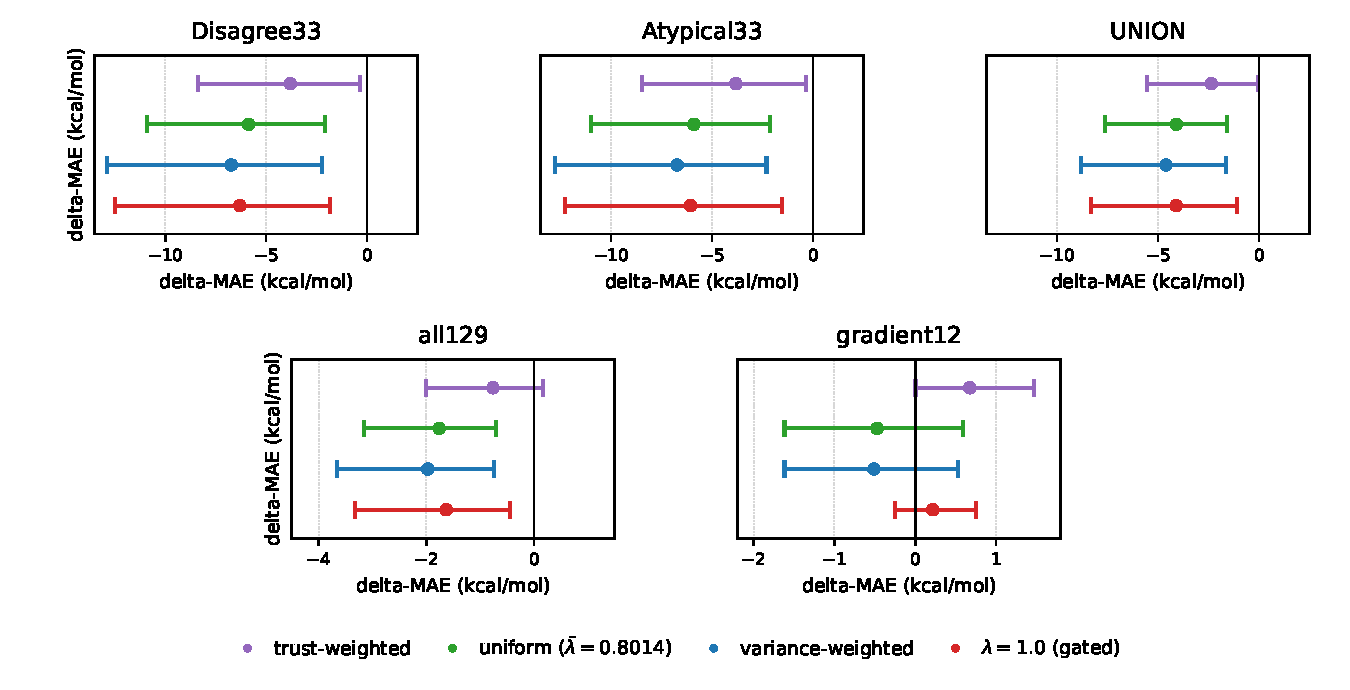
\includegraphics[width=0.88\textwidth]{fig_arms_forest.pdf}
  \caption{Forest plot of the four correction arms of
  Table~\ref{tab:arms}. Per-arm $\Delta$MAE (kcal/mol) against the
  uncorrected ensemble mean on the five fold-0 populations, with
  10{,}000 paired-bootstrap 95\% confidence intervals (vertical line at
  zero; negative values are improvements). Built directly from the archived
  arm-level result records.}
  \label{fig:arms-forest}
\end{figure} 

\section{Extended shrinkage-target search}
\label{app:shrinkage-search}

All six alternative designs operate at atom level, and through the gauge lens they are structurally capped. The variance-weighted arm's target was held fixed at the global pool mean, and six atom-level alternatives were tested.
They used the same frozen 102-molecule validation set. They used the same
five fold-0 test populations, and they used the same 10{,}000-draw paired
bootstrap. Each was calibrated on validation, and each was re-verified on the H2
holdout. (1) \emph{Variance-moderated} shrinkage. It generalizes the
$\lambda = \sigma^2/(\sigma^2+\tau^2)$ form with a per-atom magnitude cutoff
$d_0$, and its calibrated optimum is $d_0 = 0$. So it reduces algebraically to
the variance-weighted arm. (2)
\emph{Element-conditional target}, and per-element pool means replace the global
mean. The target does not contain the global arm as a boundary case, and it
underperforms it (val $-$1.645 vs $-$1.642, significantly worse on test). (3)
\emph{Two-stage within-molecule covariance}. A second, molecule-level
shrinkage targets $N_m \mu$, and it uses the actual three-seed molecular
variance. That variance is genuinely $2$--$3.5\times$ the sum of per-atom
variances, and at its calibrated optimum the second stage is a no-op. It reduces
to the variance-weighted arm, and any active pull degrades validation
monotonically.
(4) \emph{Magnitude-adaptive (James--Stein) target}. Large-deviation atoms
are shrunk less. $\lambda_i = \sigma^2_i/(\sigma^2_i + \tau^2(1+z_i^2/\eta^2))$.
The validation optimum is the $\eta^2 \to \infty$ limit, and that is the
variance-weighted arm. Large-deviation atoms are if anything slightly noisier
($\mathrm{corr}(\log|z|, \log \sigma) = +0.15$). (5) \emph{Hierarchical
element-conditional target}, and element means are themselves shrunk toward the
global mean by their seed noise.
$\mu_i = \lambda_e \mu + (1-\lambda_e)\mu_e$. This is the only design to beat
the variance-weighted arm on validation ($-2.427$ vs $-2.398$ kcal/mol). The
win reversed sign on test ($+0.04$--$+0.08$ kcal/mol worse on all five
populations). The interior optimum did not survive H1 recalibration, and we
diagnose it as overfitting to the 102-molecule validation set. (6)
\emph{Correlation-aware joint shrinkage}. A single calibrated scalar $c$
regularizes the per-molecule covariance of raw per-atom predictions.
$\hat{x} = \mu + c(\Sigma_{\mathrm{reg}} + cI)^{-1}(P - \mu)$. The estimator
$\Sigma_{\mathrm{reg}}$ is LW-regularized and block-diagonal, and under H1
recalibration its optimum is exactly $c^* = \tau^{2*} = 4.725\times 10^{-4}$.
So it reduces algebraically to the variance-weighted arm. The raw premise is
substantial within-molecule cross-seed correlation (median
$|\mathrm{corr}| = 0.83$, IQR $0.50$--$0.97$ before regularization). Even
so, it underperforms vw on validation ($-2.288$ vs $-2.398$ kcal/mol).
Detailed per-design records are archived in the project's internal
verification records and are available as part of the supplementary material.

\section{Gauge-invariant ablations}
\label{app:gims-ablations}

Three follow-up GIMS variants test the limits of invariance, and all three are reported as
negative or supporting ablations. They do not change the headline.

\textbf{GIMS-total.} This variant uses only the variance of the observable
molecular total. It defines $\Lambda_m^{\mathrm{total}}=
\operatorname{Var}_k(E_m^{(k)})/(\operatorname{Var}_k(E_m^{(k)})+\tau_E^2)$.
It uses no atomic variances at all. It is therefore invariant to any atomic
reallocation that preserves each seed's molecular total. This is a stronger
invariance. Performance is slightly worse. Test all129 is $-1.95$ vs GIMS
$-2.00$. H2 all129 is $-2.85$ vs GIMS $-2.94$. GIMS-total minus GIMS is
$+0.06$ [$-$0.04,$+$0.17] on test and $+0.09$ [$-$0.03,$+$0.23] on H2. Gradient-12
H2 has only five molecules there and is unstable. GIMS-total remains a useful
theoretical ablation. GIMS is the primary method. Its atomic variances are
used only to build a molecule-level coefficient.
% VERIFIED. GIMS-total -1.9456 vs GIMS -2.0038 test all129 and H2 -2.85 vs -2.94 = gims_report.json gims_total vs gims_train and GAUGE_INVARIANT_SHRINKAGE_RESULTS.md; diff +0.06 and +0.09 as above.

\textbf{GIMS/VW blend.} The blend is $E_{\mathrm{blend}}=(1-\alpha)E_{\mathrm{GIMS}}+
\alpha E_{\mathrm{VW}}$, and validation selects $\alpha=0.75$. H1 selects
$\alpha=0.80$ and the blend leans toward VW. It is not significant, and blend vs VW
is $-0.028$ [$-$0.067,$+$0.006] on all129 and $-0.046$ [$-$0.115,$+$0.007] on H2.
Blend vs GIMS is $+0.052$ [$-$0.037,$+$0.146] and $+0.053$ [$-$0.078,$+$0.193].
It is worse than GIMS in point estimate. It is a negative ablation.
% VERIFIED. blend alpha 0.75 val and 0.80 H1, blend vs VW -0.028 and -0.046, vs GIMS +0.052/+0.053 = node_refinement/gauge_invariant_shrinkage/gims_vw_blend_report.json and gims_vw_blend_results.csv and GAUGE_INVARIANT_SHRINKAGE_RESULTS.md Final Interpretation.

\textbf{CAAT.} Composition-Aware Affine Transfer extends the Exp-DB affine
fix with per-element terms: $\tilde E_m=aE_m+b_0+\sum_e b_e N_e$,
$N_e=\sum_i\mathbb{I}(e_i=e)$ (C, O, N, H, S, F, Cl, Br, P). Since
$\sum_i g_{mi}=0$ leaves each $N_e$ invariant, CAAT respects the same gauge
as GIMS (L2 $10^{-4}$ on $b_e$, same splits; a sweep from $10^{-2}$ to
$10^{-6}$ finds $10^{-3}$ marginally better, not grid-selected). It beats
plain affine on all three populations (5-fold CV: $-0.177$
[$-$0.244,$-$0.109] all620, $-0.310$ [$-$0.494,$-$0.123] $Q_{\rm spread}$,
$-1.16$ [$-$1.40,$-$0.94] WDec10), but against a size-matched, element-blind
control ($aE+b_0+b_N N_m$, same flexibility, no element information) it is
significant only on the two hardest populations, not on all620 ($-0.041$
[$-$0.088,$+$0.008], NS). The coefficients with the largest fold-to-fold
swings (P, Br) are also fit on the thinnest support (8--17 molecules per
fold), so whether the tail gain reflects element-specific chemistry or
flexibility concentrated on a few rare, hard molecules is unresolved.
Reported as a directional, not yet conclusive, extension.
% VERIFIED. CAAT all620/Q_spread/WDec10 = node_refinement/composition_aware_affine/composition_aware_results.csv; size-only control and coefficient stability/support = node_refinement/caat_diagnostics/CAAT_DIAGNOSTICS_REPORT.md.

Full tables for the permutation control and the train-only vs pooled
reconciliation are in the additional-checks records. They are summarized in
Results, and the underlying permutation null (5000 draws) and three-way
reconciliation tables are included in the supplementary material.
% VERIFIED. permutation and reconciliation tables = node_refinement/gauge_invariant_shrinkage/gims_additional_checks.json and docs/progress/GIMS_ADDITIONAL_CHECKS_RESULTS.md.

\section{Bias--variance decomposition of the shrinkage gain}
\label{app:bias-var}

In MSE space the shrinkage gain decomposes exactly per molecule, and it has a
bias-squared term and a variance term. Through the covariance identity of Methods, VW\textendash GIMS $=-N_m\operatorname{Cov}_i(\lambda_{mi},P_{mi})$, the small VW\textendash uniform gap is explained. It lives in variance, not bias and the identity
$\mathrm{MSE}_m = b_m^2 + v_m$ holds to machine precision for every arm and
molecule. On the four main populations, roughly two-thirds of each arm's
reduction comes from bias-squared. The share is arm-agnostic (0.65--0.67).
The remaining third is variance reduction and the arms differ sharply in how
much variance survives. On all129, vw and constant-gated shrinkage leave
$v \approx 0.3$--$0.7$ (kcal/mol)$^2$, and uniform leaves 2.6. Trust leaves 6.1.
gradient-12 is the exception, and bias-squared dominates so thoroughly that
uniform and vw show fractions above 1. Their variance slightly increases.
The two gated arms increase MSE outright, and table~\ref{tab:bias-var} gives the
full per-arm, per-population decomposition. The decomposition is in MSE
space, and it is distinct from the MAE-space deltas of Table~\ref{tab:arms}.

\begin{table}[htbp]
  \caption{Bias--variance decomposition of the shrinkage gain per arm and
  population, in (kcal/mol)$^2$. $b^2$ and $v$ are the post-correction
  bias-squared and variance; $\Delta$MSE is the change in mean squared error
  (negative is an improvement); the final column is the fraction of the MSE
  reduction attributable to bias-squared, undefined (--) where MSE
  increased. Arm abbreviations. trust, trust-weighted refinement; uniform,
  all-atom uniform at $\bar\lambda{=}0.8014$; vw, variance-weighted; gated,
  constant-$\lambda=1.0$ top-quartile gate.}
  \label{tab:bias-var}
  \centering
  \renewcommand{\arraystretch}{1.30}
  \small
  \setlength{\tabcolsep}{2pt}
  \begin{tabular}{llrrrrr}
    \toprule
    arm & population & $n$ & $b^2$ & $v$ & $\Delta$MSE & $b^2$ frac. \\
    \midrule
    trust & Q\_std & 33 & 73.85 & 23.47 & $-408.73$ & 0.655 \\
    trust & Q\_nll & 33 & 80.01 & 23.32 & $-411.35$ & 0.659 \\
    trust & UNION & 50 & 64.20 & 15.52 & $-269.64$ & 0.655 \\
    trust & all129 & 129 & 32.86 & 6.10 & $-103.25$ & 0.650 \\
    trust & gradient-12 & 12 & 18.85 & 0.12 & $+2.90$ & -- \\
    \midrule
    uniform & Q\_std & 33 & 38.16 & 8.18 & $-459.71$ & 0.660 \\
    uniform & Q\_nll & 33 & 45.07 & 7.82 & $-461.77$ & 0.663 \\
    uniform & UNION & 50 & 37.58 & 5.55 & $-306.24$ & 0.664 \\
    uniform & all129 & 129 & 19.86 & 2.61 & $-119.75$ & 0.669 \\
    uniform & gradient-12 & 12 & 10.18 & 0.67 & $-5.21$ & 1.089 \\
    \midrule
    vw & Q\_std & 33 & 27.17 & 0.87 & $-478.01$ & 0.658 \\
    vw & Q\_nll & 33 & 34.00 & 0.55 & $-480.12$ & 0.661 \\
    vw & UNION & 50 & 30.11 & 0.74 & $-318.51$ & 0.662 \\
    vw & all129 & 129 & 16.68 & 0.73 & $-124.81$ & 0.668 \\
    vw & gradient-12 & 12 & 9.61 & 0.62 & $-5.83$ & 1.071 \\
    \midrule
    gated & Q\_std & 33 & 29.51 & 0.45 & $-476.09$ & 0.656 \\
    gated & Q\_nll & 33 & 38.43 & 0.29 & $-475.96$ & 0.657 \\
    gated & UNION & 50 & 34.15 & 0.38 & $-314.83$ & 0.656 \\
    gated & all129 & 129 & 19.60 & 0.27 & $-122.35$ & 0.657 \\
    gated & gradient-12 & 12 & 16.20 & 0.14 & $+0.28$ & -- \\
    \bottomrule
  \end{tabular}
\end{table}

\newpage

%%%%%%%%%%%%%%%%%%%%%%%%%%%%%%%%%%%%%%%%%%%%%%%%%%%%%%%%%%%%

\newpage
\input{checklist.tex}

\end{document}
